\documentclass{jarticle}

\title{WiLIで用いるなくしもの位置推定の理論について}
\author{品川風丸}

\usepackage{amsmath,amssymb}
\usepackage{amsthm}
\usepackage{mathrsfs}
\usepackage{url}
\usepackage{here}
\usepackage{comment}
\usepackage{bm}
\usepackage[dvipdfmx]{graphicx}

\numberwithin{equation}{section}
\numberwithin{table}{section}
\numberwithin{figure}{section}

\theoremstyle{plain}
\newtheorem{joken}{条件}

\begin{document}

\maketitle

\section{はじめに}
本ファイルではWiLIに用いるなくしもの位置推定の理論について述べる。
またREADME.mdはですます調で書かれているが、本ファイルは数学に関する内容が主であることを踏まえだである調で書く。

なくしものの位置を推定するにあたり、まずなくしものの発生の原理について考える。
経験則としてなくしものはある動作から別の動作へ移る際に手に持っているものを置く場合に発生しやすい。
例えば筆者の実体験として、郵便受けから新聞紙を取ろうと手に持っていたスマホを床に置いてそのまま忘れる等がある。
WiLIではこの経験則をもとに利用者の行動を確率論を用いてモデル化し、その下でなくしものの位置の確率分布を計算する。


\section{理論}

\subsection{概要}
利用者の行動について以下の2つの仮定を敷く。
\begin{itemize}
    \item 仮定1:利用者は動作をノードとするマルコフ連鎖に従う。
    \item 仮定2:ある動作から別の動作へ遷移する際に確率的になくしものが発生する。またこの際の確率は遷移先の動作にのみ依存するとし、その確率を遷移失敗確率と呼ぶ。
\end{itemize}
この仮定の下では遷移を繰り返すといつかはなくしものが発生する。
さらに各動作ごとになくしものが発生した際に遷移先がその動作であった確率を計算できる。この確率をなくしもの発生確率と呼ぶ。

ここで各動作ごとに利用者がその動作下でどこにいるかの傾向を表す位置分布を用意し、
全動作に渡り利用者の位置分布をなくしもの発生確率を重みとして足し合わせる。
こうして得られた分布はなくしものが発生した際に利用者がいた位置の確率分布を表していると考えられる。
そこでこの分布をなくしものの位置の確率分布とみなす。


\subsection{定式化}
表\ref{tbl:f_symbol}のように記号を置く。

\begin{center}
    \begin{table}[h]
        \caption{記号}
        \label{tbl:f_symbol}

        \begin{tabular}{c|l}
            記号 & 概要 \\
            \hline \hline

            % 基本的な記号
            $X$ & \begin{tabular}{l}
                捜索範囲 \\
                $ \mathbb{R}^2 $または$ \mathbb{R}^3 $の部分集合
            \end{tabular} \\

            \hline
            $n$ & \begin{tabular}{l}
                動作の数 \\
                \ (利用者が従うマルコフ連鎖のノードの数)
            \end{tabular} \\

            \hline
            $M_i(i=1,2,\cdots,n)$ & \begin{tabular}{l}
                $i$番目の動作
            \end{tabular} \\

            \hline
            $m_t(t=0,1,2,\cdots)$ & \begin{tabular}{l}
                $t$回目の遷移を終えた直後の動作 \\
                ただし$m_0$は初期動作とする
            \end{tabular} \\

            \hline
            $\mathrm{LI}$ & \begin{tabular}{l}
                なくしものが発生したことを表す
            \end{tabular} \\

            \hline
            $\mathrm{NLI}$ & \begin{tabular}{l}
                なくしものが発生しなかったことを表す
            \end{tabular} \\

            \hline
            $r_t(t=1,2,\cdots)$ & \begin{tabular}{l}
                $t$回目の遷移でなくしものが発生した場合は$\mathrm{LI}$を、\\
                発生しなかった場合は$\mathrm{NLI}$を返す確率変数
            \end{tabular} \\

            \hline
            $\tau$ & \begin{tabular}{l}
                次を満たす数 \\
                任意の$t < \tau$に対し$r_t=\mathrm{NLI}$かつ$r_\tau=\mathrm{LI}$ \\
                \ ($\tau$回目までの遷移ではなくしものが発生せず、\\$\tau$回目の遷移で発生する)
            \end{tabular} \\

            % パラメータ
            \hline
            $s_i$ & \begin{tabular}{l}
                初期動作が$M_i$である確率 \\
                $\mathrm{P}(m_0=M_i)$
            \end{tabular} \\
        \end{tabular}
    \end{table}
\end{center}

これらの記号の下、仮定1と仮定2加えて利用者の位置分布を次のように定式化する。
\begin{joken}[仮定1]
    $ \mathrm{P}(m_{t+1}=M_j\ |\ m_t=M_i) $は$i$と$j$にのみ依存する。
    この確率は$M_i$から$M_j$への遷移確率と呼び$a_{i j}$と書く。
\end{joken}

\begin{joken}[仮定2]
    $t$に依らず次式が成り立つ。
    \begin{equation}
        \mathrm{P}(r_{t+1} = \mathrm{LI}\ |\ m_{t+1}=m_t) = 0
    \end{equation}
\end{joken}

\begin{joken}[仮定2]
    $ \mathrm{P}(r_{t+1} = \mathrm{LI}\ |\ m_{t+1}=M_i , m_{t+1} \ne m_t) $は$i$にのみ依存する。
    この確率を$M_i$への遷移失敗確率と呼び$\theta_i$と書く。
\end{joken}

\begin{joken}[利用者の位置分布]
    $M_i$に$X$上の確率分布が付随しているとし、その密度関数を$ b_i:X\rightarrow\mathbb{R} $と書く。
\end{joken}
また$M_i$でのなくしもの発生確率$p_i(i=1,2,\cdots,n)$を次式で定める。
\begin{equation}
    \label{eq:p_def}
    p_i =\mathrm{P}(\tau < \infty , m_\tau = M_i)
\end{equation}

$p_i$は$a_{i j}$、$s_i$、$\theta_i$を用いれば式(\ref{eq:p})のように表せる。
導出は補足として\ref{sec:calc_p}章に書く。
\begin{equation}
    \label{eq:p}
    \bm{p} =\bm{L}(\bm{I} - \bm{K})^{-1}\bm{s}
\end{equation}
\begin{align*}
    \bm{p} &= (p_1\ p_2\ \cdots\ p_n)^\mathrm{T} \\
    \bm{L} &= \begin{pmatrix}
        0                & \theta_1 a_{1 2} & \cdots & \theta_1 a_{1 n} \\
        \theta_2 a_{2 1} & 0                &        & \theta_2 a_{2 n} \\
        \vdots           &                  & \ddots & \vdots           \\
        \theta_n a_{n 1} & \theta_n a_{n 2} & \cdots & 0
    \end{pmatrix} \\
    \bm{I} & \quad \ \text{$n$行$n$列の単位行列} \\
    \bm{K} &= \begin{pmatrix}
                       a_{1 1} & (1 - \theta_1) a_{1 2} & \cdots & (1 - \theta_1) a_{1 n} \\
        (1 - \theta_2) a_{2 1} &                a_{2 2} &        & (1 - \theta_2) a_{2 n} \\
        \vdots                 &                        & \ddots & \vdots                 \\
        (1 - \theta_n) a_{n 1} & (1 - \theta_n) a_{n 2} & \cdots &                a_{n n}
    \end{pmatrix} \\
    \bm{s} &= (s_1\ s_2\ \cdots\ s_n)^\mathrm{T} \\
\end{align*}

備考として$\bm{L}$と$\bm{K}$は$a_{i j}$に対し次式を満たす。
\begin{equation}
    \label{eq:L+K=A}
    \bm{L} + \bm{K} = \begin{pmatrix}
        a_{1 1} & a_{1 2} & \cdots & a_{1 n} \\
        a_{2 1} & a_{2 2} &        & a_{2 n} \\
        \vdots  &         & \ddots & \vdots  \\
        a_{n 1} & a_{n 2} & \cdots & a_{n n}
    \end{pmatrix}
\end{equation}

なくしもの位置の確率分布を$p_i$と$b_i$を用いて次式の関数$ h \! : \! X /! \rightarrow \! \mathbb{R}$を密度関数としてもつような分布として定める。
\begin{equation}
    \label{eq:h}
    h = \sum_{i} {p_i b_i}
\end{equation}


\subsection{パラメータ学習方法}
必要なパラメータは遷移確率$a_{i j}$、初期確率$s_i$、遷移失敗確率$\theta_i$、利用者の位置分布$b_i$の4種である。

このうち$a_{i j}$、$s_i$、$b_i$について、これらはマルコフ連鎖の各ノードに確率分布が付随しているという点で隠れマルコフモデル(以下HMM)に類似している。
そのため利用者の位置分布を正規分布に限定すれば、
利用者の位置推移からHMMの学習アルゴリズムによりパラメータの学習が可能であると考えられる。

残る$\theta_i$はベイズ推定により学習する。
$\bm{\theta} = (\theta_1\ \theta_2\ \cdots\ \theta_n)^\mathrm{T}$が従う確率分布の密度関数$f:[0,1]^n \rightarrow \mathbb{R}$を
真のなくしもの位置$\bm{x}_\mathrm{true} \in X$を用いて式(\ref{eq:update_theta})により更新する。
\begin{equation}
    \label{eq:update_theta}
    f(\bm{\theta} | \bm{x}_\mathrm{true}) \propto h(\bm{x}_\mathrm{true} | \bm{\theta}) f(\bm{\theta})
\end{equation}


\subsection{なくしもの位置の推定方法}
遷移失敗確率$\theta_i$の学習は点推定ではなく分布を推定している。
そこでなくしもの位置の推定結果としてなくしもの位置の確率分布の$\bm{\theta}$に関する平均値、
すなわち次式を密度関数としてもつ確率分布を採用する。
\begin{equation}
    \label{eq:Eh}
    \mathrm{E}_{\bm{\theta}} \left[ h \right]\ :\ 
    \begin{aligned}[t]
        X &\rightarrow \mathbb{R} \\
        \bm{x} &\mapsto \int {h(\bm{x} | \bm{\theta}) f(\bm{\theta}) \mathrm{d} \bm{\theta}}
    \end{aligned}
\end{equation}


\section{補足:なくしもの発生確率の導出}
\label{sec:calc_p}
本章では式(\ref{eq:p})の導出をする。

まず$ p_{t i} = \mathrm{P}(\tau = t\ , m_\tau = M_i) $とおく。これはなくしもの発生確率$p_i$に対し次式を満たす。
\begin{equation} \label{eq:pi=sum_pti}
    p_i = \sum_{t=1}^{\infty}p_{t i}
\end{equation}
また$ \bm{p}_{t} = (p_{t 1}\ p_{t 2}\ \cdots\ p_{t n})^\mathrm{T} $とおけば次のようにも書ける。
\begin{equation} \label{eq:p=sum_pt}
    \bm{p} = \sum_{t=1}^{\infty} \bm{p}_{t i}
\end{equation}
そこで式(\ref{eq:p})を導くために$ p_{t i} $の$t$に関する一般項を求める。

$ p_{t i} $の一般項を求めるにあたって$ q_{t i} = \mathrm{P}(\tau > t\ , m_t=M_i) $の一般項を求める。
$ q_{t i} $は次の漸化式を満たす。
\begin{align}
    q_{t+1\ i} & = \! \sum_{k} \mathrm{P}(\tau \! > \! t + 1\ , m_{t+1} \! = \! M_i\ , m_t \! = \! M_k) \nonumber\\
    & = \! \sum_{k} \mathrm{P}(\tau \! \ne \! t + 1 , m_{t+1} \! = \! M_i , m_t \! = \! M_k | \tau \! > \! t) \mathrm{P}(\tau \! > \! t) \nonumber\\
    & = \! \sum_{k} \left(
        \begin{array}{l}
            \mathrm{P}(\tau \! \ne \! t + 1 | \tau \! > \! t , m_{t+1} \! = \! M_i , m_t \! = \! M_k) \\
            \times \mathrm{P}(m_{t+1} \! = \! M_i , m_t \! = \! M_k | \tau \! > \! t) \mathrm{P}(\tau \! > \! t)
        \end{array}
     \right) \nonumber\\
    & = \! \sum_{k} \left(
        \begin{array}{l}
            \mathrm{P}(r_t \! = \! \mathrm{NLI} | \forall t' \! \le \! t \ \mathrm{s.t.}\ r_{t'}\! =\!\mathrm{NLI} , m_{t+1} \! = \! M_i , m_t \! = \! M_k) \\
            \times \mathrm{P}(m_{t+1} \! = \! M_i , m_t \! = \! M_k) \mathrm{P}(\tau \! > \! t)
        \end{array}
    \right) \nonumber\\
    & = \! \sum_{k} \left(
        \begin{array}{l}
            \mathrm{P}(r_t \! = \! \mathrm{NLI} | m_{t+1} \! = \! M_i , m_t \! = \! M_k) \\
            \times \mathrm{P}(m_{t+1} \! = \! M_i | m_t \! = \! M_k) \mathrm{P}(m_t \! = \! M_k) \mathrm{P}(\tau \! > \! t)
        \end{array}
    \right) \nonumber\\
    & = \! \sum_{k} \left(
        \begin{array}{l}
            \mathrm{P}(r_t \! = \! \mathrm{NLI} | m_{t+1} \! = \! M_i , m_t \! = \! M_k) \\
            \times \mathrm{P}(m_{t+1} \! = \! M_i | m_t \! = \! M_k) \mathrm{P}(\tau \! > \! t , m_t \! = \! M_k)
        \end{array}
    \right) \nonumber\\
    & = \! \sum_{k \ne i} (1 - \theta_i) a_{k i} q_{t k} + a_{i i} q_{t i} \label{eq:qti_rec}
\end{align}
この式(\ref{eq:qti_rec})は$ \bm{q}_t = (q_{t 1}\ q_{t 2}\ \cdots\ q_{t n})^\mathrm{T} $とおけば次式のようにも書ける。
\begin{equation}
    \arraycolsep3pt
    \bm{q}_{t + 1} \! = \!
    \begin{pmatrix}
        a_{1 1} & (1 \! - \! \theta_1) a_{2 1} & \cdots & (1 \! - \! \theta_1) a_{n 1} \\
        (1 \! - \! \theta_2) a_{1 2} & a_{2 2} & \cdots & (1 \! - \! \theta_2) a_{n 2} \\
        \vdots & \vdots & \ddots & \vdots \\
        (1 \! - \! \theta_n) a_{1 n} & (1 \! - \! \theta_n) a_{2 n} & \cdots & a_{n n} \\
    \end{pmatrix}
    \! \bm{q}_t
    \label{eq:qt_rec}
\end{equation}
式(\ref{eq:qt_rec})の係数行列を$ \bm{K} $とおく。
一方初項$ q_{1 i} $についても$ \mathrm{P}(\tau > 0) = 1 $であることに注意すれば式(\ref{eq:qti_rec})と同様にして次式を得る。
\begin{align}
    q_{1 i} & = \! \sum_{k} \left(
        \begin{array}{l}
            \mathrm{P}(r_1 = \mathrm{NLI}\ |\ m_1 = M_i , m_0 = M_k) \\
            \times \mathrm{P}(m_1 = M_i\ |\ m_0 = M_k) \mathrm{P}(m_0 = M_k)
        \end{array}
    \right) \nonumber\\
    & = \! \sum_{k \ne i} (1 - \theta_i) a_{k i} s_k + a_{i i} s_i
    \label{eq:q1i}
\end{align}
この式(\ref{eq:q1i})は$ \bm{s} = (s_1\ s_2\ \cdots\ s_n)^\mathrm{T} $と$ \bm{K} $を使えば次式のようになる。
\begin{equation} \label{eq:qt_init}
    \bm{q}_1 = \bm{K} \bm{s}
\end{equation}
よって式(\ref{eq:qt_rec})、(\ref{eq:qt_init})から$ \bm{q}_t $の一般項は次式となる。
\begin{equation} \label{eq:qt}
    \bm{q}_t = \bm{K}^t \bm{s}
\end{equation}

次に$ p_{t i} $の一般項について、式(\ref{eq:qti_rec})と同様にして次式を得る。
\begin{align}
    p_{t+1\ i} & = \! \sum_{k} \mathrm{P}(\tau = t + 1 , \sigma_{t+1} = S_i , \sigma_t = S_k) \nonumber\\
    & = \! \sum_{k} \left(
        \begin{array}{l}
            \mathrm{P}(r_t = \mathrm{LI}\ |\ m_{t+1} \! = \! M_i , m_t \! = \! M_k) \\
            \times \mathrm{P}(m_{t+1} \! = \! M_i\ |\ m_t \! = \! M_k) \mathrm{P}(\tau \! > \! t , m_t \! = \! M_k)
        \end{array}
    \right) \nonumber\\
    & = \! \sum_{k \ne i} \theta_i a_{k i} q_{t k}
    \label{eq:pti_rec}
\end{align}
この式(\ref{eq:pti_rec})は$ \bm{p}_t $を使えば次のようになる。
\begin{equation}
    \arraycolsep3pt
    \bm{p}_{t + 1} = 
    \begin{pmatrix}
        0 & \theta_1 a_{2 1} & \cdots & \theta_1 a_{n 1} \\
        \theta_2 a_{1 2} & 0 & \cdots & \theta_2 a_{n 2} \\
        \vdots & \vdots & \ddots & \vdots \\
        \theta_n a_{1 n} & \theta_n a_{2 n} & \cdots & 0 \\
    \end{pmatrix}
    \bm{q}_t
\end{equation}
この係数行列を$ \bm{L} $とおき式(\ref{eq:qt})を代入すれば次式を得る。
\begin{equation} \label{eq:pt}
    \bm{p}_t = \bm{L} \bm{K}^{t - 1} \bm{s}
\end{equation}

\begin{figure}[bt]
    \centering
    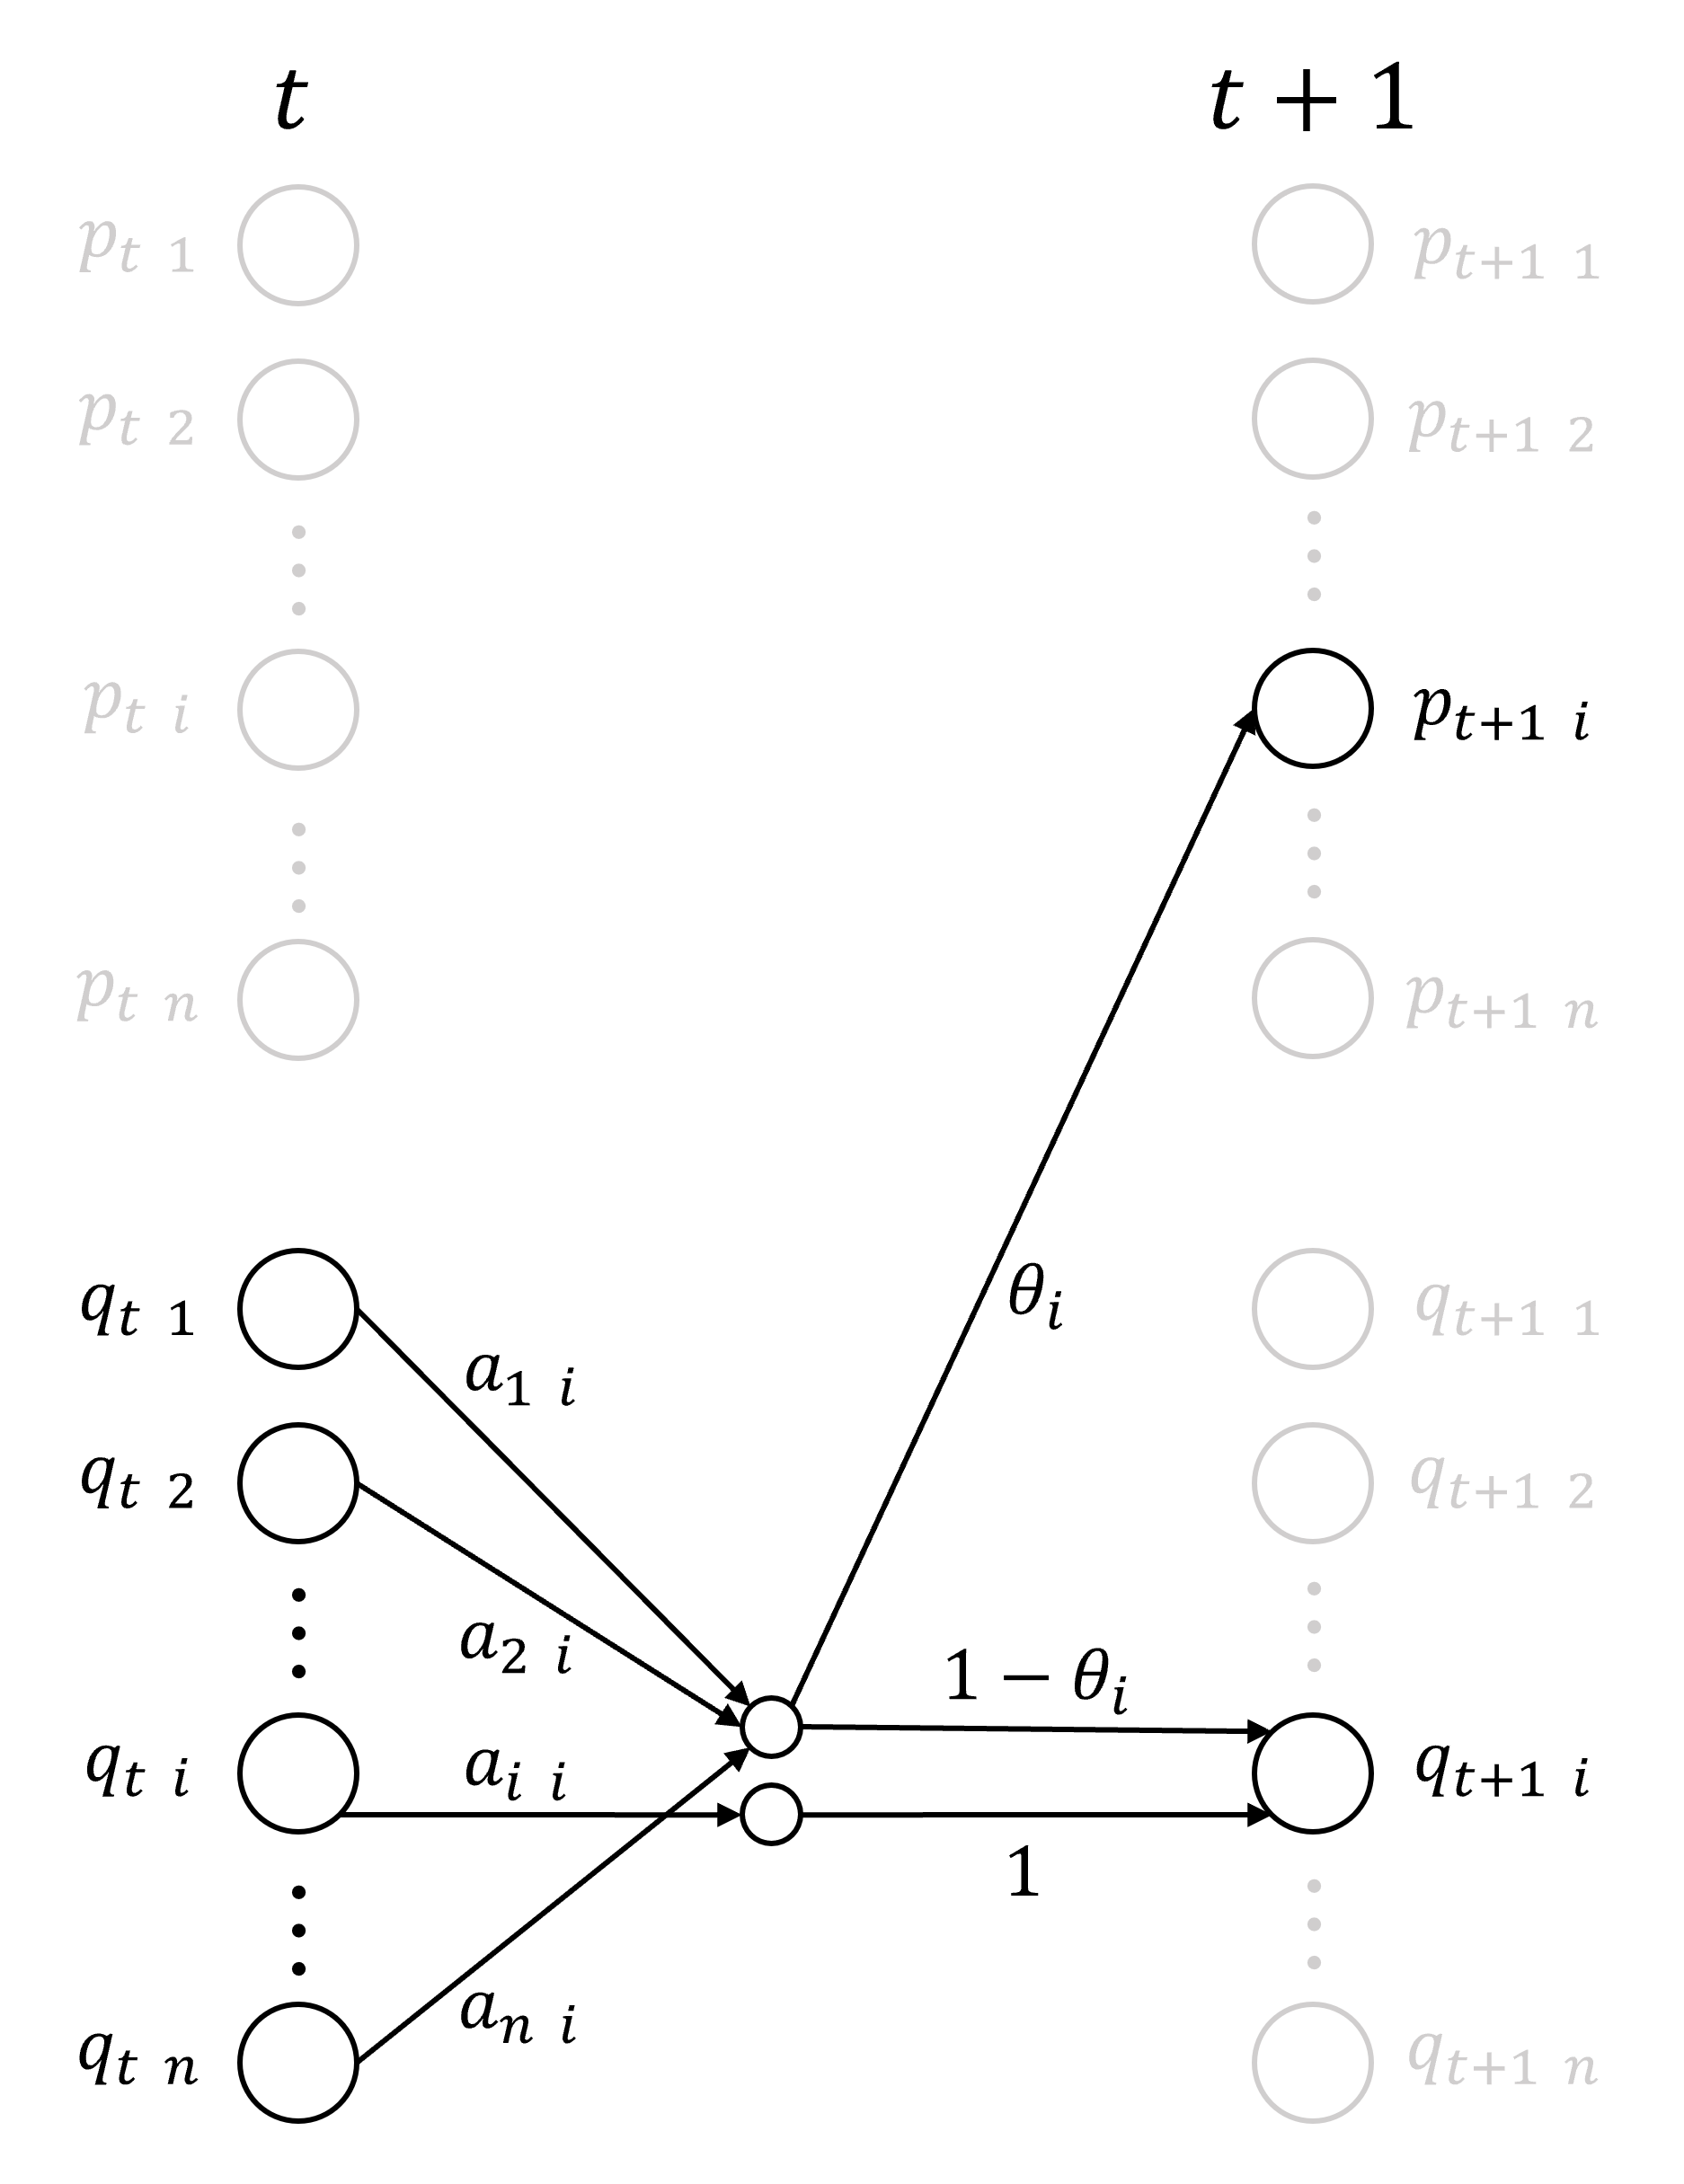
\includegraphics[keepaspectratio, width=0.7\linewidth]{img/pq.eps}
    \caption{$ p_{t i} $と$ q_{t i} $の漸化式のイメージ}
\end{figure}

$ \bm{p}_t $の一般項が求まったので次に$ \bm{p} $について求める。式(\ref{eq:pt})を式(\ref{eq:p=sum_pt})に代入すると次のようになる。
\begin{align}
    \bm{p} &= \sum_{t=1}^{\infty} \bm{L} \bm{K}^{t - 1} \bm{s} \nonumber \\
    &= \bm{L} \left( \sum_{t=0}^{\infty} \bm{K}^t \right) \bm{s} \label{eq:p_}
\end{align}

ここで$ \sum \bm{K}^t $が収束性について、ゲルシュゴリンの定理\cite{bib:s_saito}より$ \bm{K}^\mathrm{T} $の任意の固有値$ \lambda $はいずれかの$ i $に対し次式を満たす。
\begin{equation}
    \label{eq:lambda}
    a_{i i} - \sum_{j \ne i}(1 - \theta_j) a_{i j} \le \lambda \le a_{i i} + \sum_{j \ne i}(1 - \theta_j) a_{i j}
\end{equation}
式(\ref{eq:lambda})の右辺は次のように評価できる。
\begin{align*}
    \lambda &\le a_{i i} + \sum_{j \ne i}(1 - \theta_j) a_{i j} \\
    &\le a_{i j} + \sum_{j \ne i} a_{i j} \\
    &= 1
\end{align*}
等号が成り立つのは任意の$j$に対し$a_{i j} > 0 \Rightarrow \theta_j = 0$が成り立つときに限る。
また式(\ref{eq:lambda})の左辺についても次のように評価できる。
\begin{align*}
    \lambda &\ge a_{i i} - \sum_{j \ne i}(1 - \theta_j) a_{i j} \\
    &\ge a_{i i} \\
    &\ge 1
\end{align*}
等号が成り立つのは$a_{i i}=1$のときに限る。
よって任意の$i$に対し$a_{i i} < 1$かつ、任意の$i$に対し適当な$j$が存在して$a_{i j} > 0$かつ$\theta_j > 0$となるとき
$ \bm{K}^\mathrm{T} $の固有値はいずれも絶対値が$ 1 $未満であり、また$ \bm{K} $と$ \bm{K}^\mathrm{T} $の固有値は等しいので$ \bm{K} $の固有値も絶対値が$ 1 $未満となる。
このとき$ \sum \bm{K}^t $は収束し収束先は行列等比級数の公式\cite{bib:m_saito}により次のように求まる。
\begin{equation} \label{eq:sumK}
    \sum_{t=0}^{\infty} \bm{K}^t = (\bm{I} - \bm{K})^{-1}
\end{equation}
ただし$ \bm{I} $は$n$行$n$列の単位行列である。

最後に式(\ref{eq:sumK})を式(\ref{eq:p_})に代入すれば式(\ref{eq:p})を得る。

\begin{thebibliography}{99}
    \bibitem{bib:s_saito}
    齊藤:数値解析学入門.pp.108--109,東京大学出版会,2012.
    \bibitem{bib:m_saito}
    齋藤:基礎数学1 線形代数入門.pp.212,東京大学出版会,1966.
\end{thebibliography}

\end{document}